%% 
%% Copyright 2019-2024 Elsevier Ltd
%% 
%% This file is part of the 'CAS Bundle'.
%% --------------------------------------
%% 
%% It may be distributed under the conditions of the LaTeX Project Public
%% License, either version 1.3c of this license or (at your option) any
%% later version.  The latest version of this license is in
%%    http://www.latex-project.org/lppl.txt
%% and version 1.3c or later is part of all distributions of LaTeX
%% version 1999/12/01 or later.
%% 
%% The list of all files belonging to the 'CAS Bundle' is
%% given in the file `manifest.txt'.
%% 
%% Template article for cas-dc documentclass for 
%% double column output.

\documentclass[a4paper,fleqn]{cas-dc}

% If the frontmatter runs over more than one page
% use the longmktitle option.

%\documentclass[a4paper,fleqn,longmktitle]{cas-dc}

%\usepackage[numbers]{natbib}
%\usepackage[authoryear]{natbib}
\usepackage[authoryear,longnamesfirst]{natbib}

%%%Author macros
\def\tsc#1{\csdef{#1}{\textsc{\lowercase{#1}}\xspace}}
\tsc{WGM}
\tsc{QE}
%%%

% Uncomment and use as if needed
%\newtheorem{theorem}{Theorem}
%\newtheorem{lemma}[theorem]{Lemma}
%\newdefinition{rmk}{Remark}
%\newproof{pf}{Proof}
%\newproof{pot}{Proof of Theorem \ref{thm}}

\begin{document}
\let\WriteBookmarks\relax
\def\floatpagepagefraction{1}
\def\textpagefraction{.001}

% Short title
\shorttitle{}    

% Short author
\shortauthors{}  

% Main title of the paper
\title [mode = title]{RouteSAM: Semantic Routing for Semi-Supervised 2D Medical Image Segmentation via Cross-Image Propagation}  


% Title footnote mark
% eg: \tnotemark[1]
\tnotemark[1] 

% Title footnote 1.
% eg: \tnotetext[1]{Title footnote text}
\tnotetext[1]{} 

% First author
%
% Options: Use if required
% eg: \author[1,3]{Author Name}[type=editor,
%       style=chinese,
%       auid=000,
%       bioid=1,
%       prefix=Sir,
%       orcid=0000-0000-0000-0000,
%       facebook=<facebook id>,
%       twitter=<twitter id>,
%       linkedin=<linkedin id>,
%       gplus=<gplus id>]

\author[1]{}%[<options>]

% Corresponding author indication
\cormark[1]

% Footnote of the first author
\fnmark[1]

% Email id of the first author
\ead{}

% URL of the first author
\ead[url]{}

% Credit authorship
% eg: \credit{Conceptualization of this study, Methodology, Software}
\credit{}

% Address/affiliation
\affiliation[1]{organization={},
            addressline={}, 
            city={},
%          citysep={}, % Uncomment if no comma needed between city and postcode
            postcode={}, 
            state={},
            country={}}

\author[2]{}%[]

% Footnote of the second author
\fnmark[2]

% Email id of the second author
\ead{}

% URL of the second author
\ead[url]{}

% Credit authorship
\credit{}

% Address/affiliation
\affiliation[2]{organization={},
            addressline={}, 
            city={},
%          citysep={}, % Uncomment if no comma needed between city and postcode
            postcode={}, 
            state={},
            country={}}

% Corresponding author text
\cortext[1]{Corresponding author}

% Footnote text
\fntext[1]{}

% For a title note without a number/mark
%\nonumnote{}

% Here goes the abstract
\begin{abstract}
Existing semi-supervised medical image segmentation methods typically treat each unlabeled image as an independent pseudo-labeling target and connect labeled and unlabeled data through model predictions, consistency constraints, or cross-image transfer. Under extreme label scarcity, however, a few labeled samples cannot adequately cover the diversity of lesion morphology, scale, and appearance. Models therefore struggle to provide reliable supervision for semantically distant unlabeled targets, while one-step cross-image transfer is also prone to failure. Once used for training, such erroneous supervision can be repeatedly reinforced and ultimately impair segmentation performance. To address this problem, we propose RouteSAM, which reformulates semi-supervised medical image segmentation under extreme label scarcity as a cross-image supervision-routing problem. Instead of requiring a limited set of labeled samples to establish difficult direct connections with all unlabeled targets, RouteSAM exploits the latent semantic continuity of the unlabeled data to plan progressive, easy-to-difficult routes for supervision propagation. In this view, unlabeled images are not only pseudo-labeling targets but also intermediate semantic nodes connecting labeled samples to difficult targets. Under a fixed annotation budget, RouteSAM first selects a small set of images that covers the training distribution as labeled Anchors. For each Target, it identifies an appropriate source, retrieves semantically continuous unlabeled Bridge images, and organizes them into an ordered Anchor--Bridge--Target route. SAM3 progressively propagates the Anchor mask along the route, decomposing a difficult transfer across a large semantic gap into a sequence of smoother local transitions and producing multiple target-mask candidates from different Anchors and route depths. To suppress route-selection errors and error accumulation, RouteSAM estimates candidate quality from the route structure and propagation process, and introduces a task-specific segmentation model to learn from reliable supervision, audit propagation results, and provide medical-domain feedback. The domain-adapted SAM3 then propagates again along the frozen routes, forming a collaborative loop of generalist supervision expansion, specialist learning and auditing, and generalist re-propagation. Semantic retrieval and route propagation are used only during training; the final model directly segments a single image without retrieving references, constructing routes, or requiring manual prompts. Experiments on Kvasir-SEG, BUSI, and ISIC2018 under an approximately 1\% annotation budget show that RouteSAM \textbf{[final quantitative results to be inserted]}, demonstrating the value of explicitly planning how supervision travels from labeled to unlabeled medical data.
\end{abstract}

% Use if graphical abstract is present
%\begin{graphicalabstract}
%\includegraphics{}
%\end{graphicalabstract}

% Research highlights
\begin{highlights}
\item RouteSAM organizes unlabeled images into ordered propagation routes.
\item Coverage-aware Anchors diversify sources under a 1\% label budget.
\item Semantic Bridges replace difficult direct transfer with progressive propagation.
\item A SAM3--U-Net loop audits and re-propagates route-derived supervision.
\item The final specialist supports prompt-free single-image inference.
\end{highlights}


%\nocite{*}

% Keywords
% Each keyword is seperated by \sep
\begin{keywords}
Semi-supervised medical image segmentation \sep
Segment Anything Model \sep
Cross-image propagation \sep
Semantic routing \sep
Pseudo-label learning
\end{keywords}

\maketitle

% Main text



\section{Introduction}

Pixel-level annotation remains a major bottleneck in medical image segmentation because accurate delineation is time-consuming and requires domain expertise. Semi-supervised medical image segmentation (SSMIS) alleviates this burden by learning from a limited labeled set together with a much larger pool of unlabeled images. Representative methods generate pseudo labels or enforce prediction consistency under input, feature, and model perturbations~\cite{tarvainen2017meanteacher,chen2021cps,luo2022crossteaching,wu2022mcnet,bai2023bcp,assefa2025dycon}. In commonly studied settings where approximately 5\%--20\% of the training data are labeled, these methods can substantially outperform supervised baselines trained on the same labeled subset, demonstrating that unlabeled data can compensate for a considerable portion of the missing annotations~\cite{luo2022crossteaching,bai2023bcp,assefa2025dycon}.

Building on this progress, promptable segmentation foundation models provide an additional way to strengthen learning with limited annotations. The Segment Anything Model (SAM) family~\cite{kirillov2023segment,ravi2025sam2,carion2026sam3} has acquired strong prompt-conditioned segmentation priors through large-scale pretraining. Although direct deployment remains unreliable because medical and natural images differ substantially in image formation, contrast, target scale, and morphology~\cite{mazurowski2023samexperiment,ma2024medsam}, SAM can still serve as a generalist prior when coupled with a task-specific medical model. Recent SAM-assisted SSMIS methods therefore use specialist predictions to prompt SAM, use SAM outputs to refine pseudo labels, or exchange knowledge between the generalist and specialist, further strengthening the supervision extracted from unlabeled images~\cite{zhang2023semisam,zhang2025semisamplus,xu2024samatch,miao2024cpcsam,vu2026scsam,zhang2026cppssam}.

However, when labeled data are reduced further, such that only a handful of images in the entire training set have pixel-level annotations, conventional semi-supervised models and promptable segmentation foundation models are more likely to produce unreliable pseudo supervision and erroneous predictions. Reusing these erroneous predictions as training supervision may further amplify confirmation bias, causing errors to accumulate over iterative training.

We observe that this phenomenon often occurs when a substantial visual or semantic gap exists between labeled source images and unlabeled target images. A limited set of labeled sources cannot adequately cover the diversity of lesion morphology, scale, and appearance. Consequently, conventional semi-supervised models may struggle to generate reliable pseudo labels for targets that differ substantially from the labeled examples, while promptable segmentation foundation models may also struggle to obtain accurate target masks from the mask prompts provided by labeled sources.

Existing methods focus primarily on the relationship between source and target images, while abundant unlabeled data and their internal relationships often remain insufficiently explored. This motivates us to ask: can latent semantic relations among unlabeled images be used to bridge the semantic gap between labeled sources and difficult targets, decomposing a direct transfer across a large semantic distance into multiple more local propagation steps?

The unlabeled pool also contains useful dataset-level structure. ACTION learns global semantic relations and local anatomical contrast~\cite{you2022action}; DACL constructs density-aware neighborhood graphs to compact class features~\cite{tang2024dacl}; and GraphCL models instance relations through graph-based clustering~\cite{wang2024graphcl}. These methods demonstrate the value of cross-sample relations, but mainly use them to regularize feature learning rather than to define an executable path for mask propagation.

More closely related work transfers masks across images under one-shot supervision. OP-SAM transfers a prior from a labeled support image to a query through feature correlation and iterative prompt evolution~\cite{mao2025opsam}. YoloSeg uses SAM2 to propagate a single labeled mask to an unlabeled pool and trains a task-specific model using multi-view consensus and divergence regions~\cite{zhang2026yoloseg}. These studies establish the value of foundation-model-driven propagation, yet the transfer is still organized around a direct support-to-query connection rather than an explicitly selected and ordered sequence of intermediate unlabeled samples. When the labeled source and target differ substantially in morphology, scale, or appearance, such a one-step transfer can remain difficult even if its output is subsequently filtered or regularized.

\begin{figure}[pos=t]
    \centering
    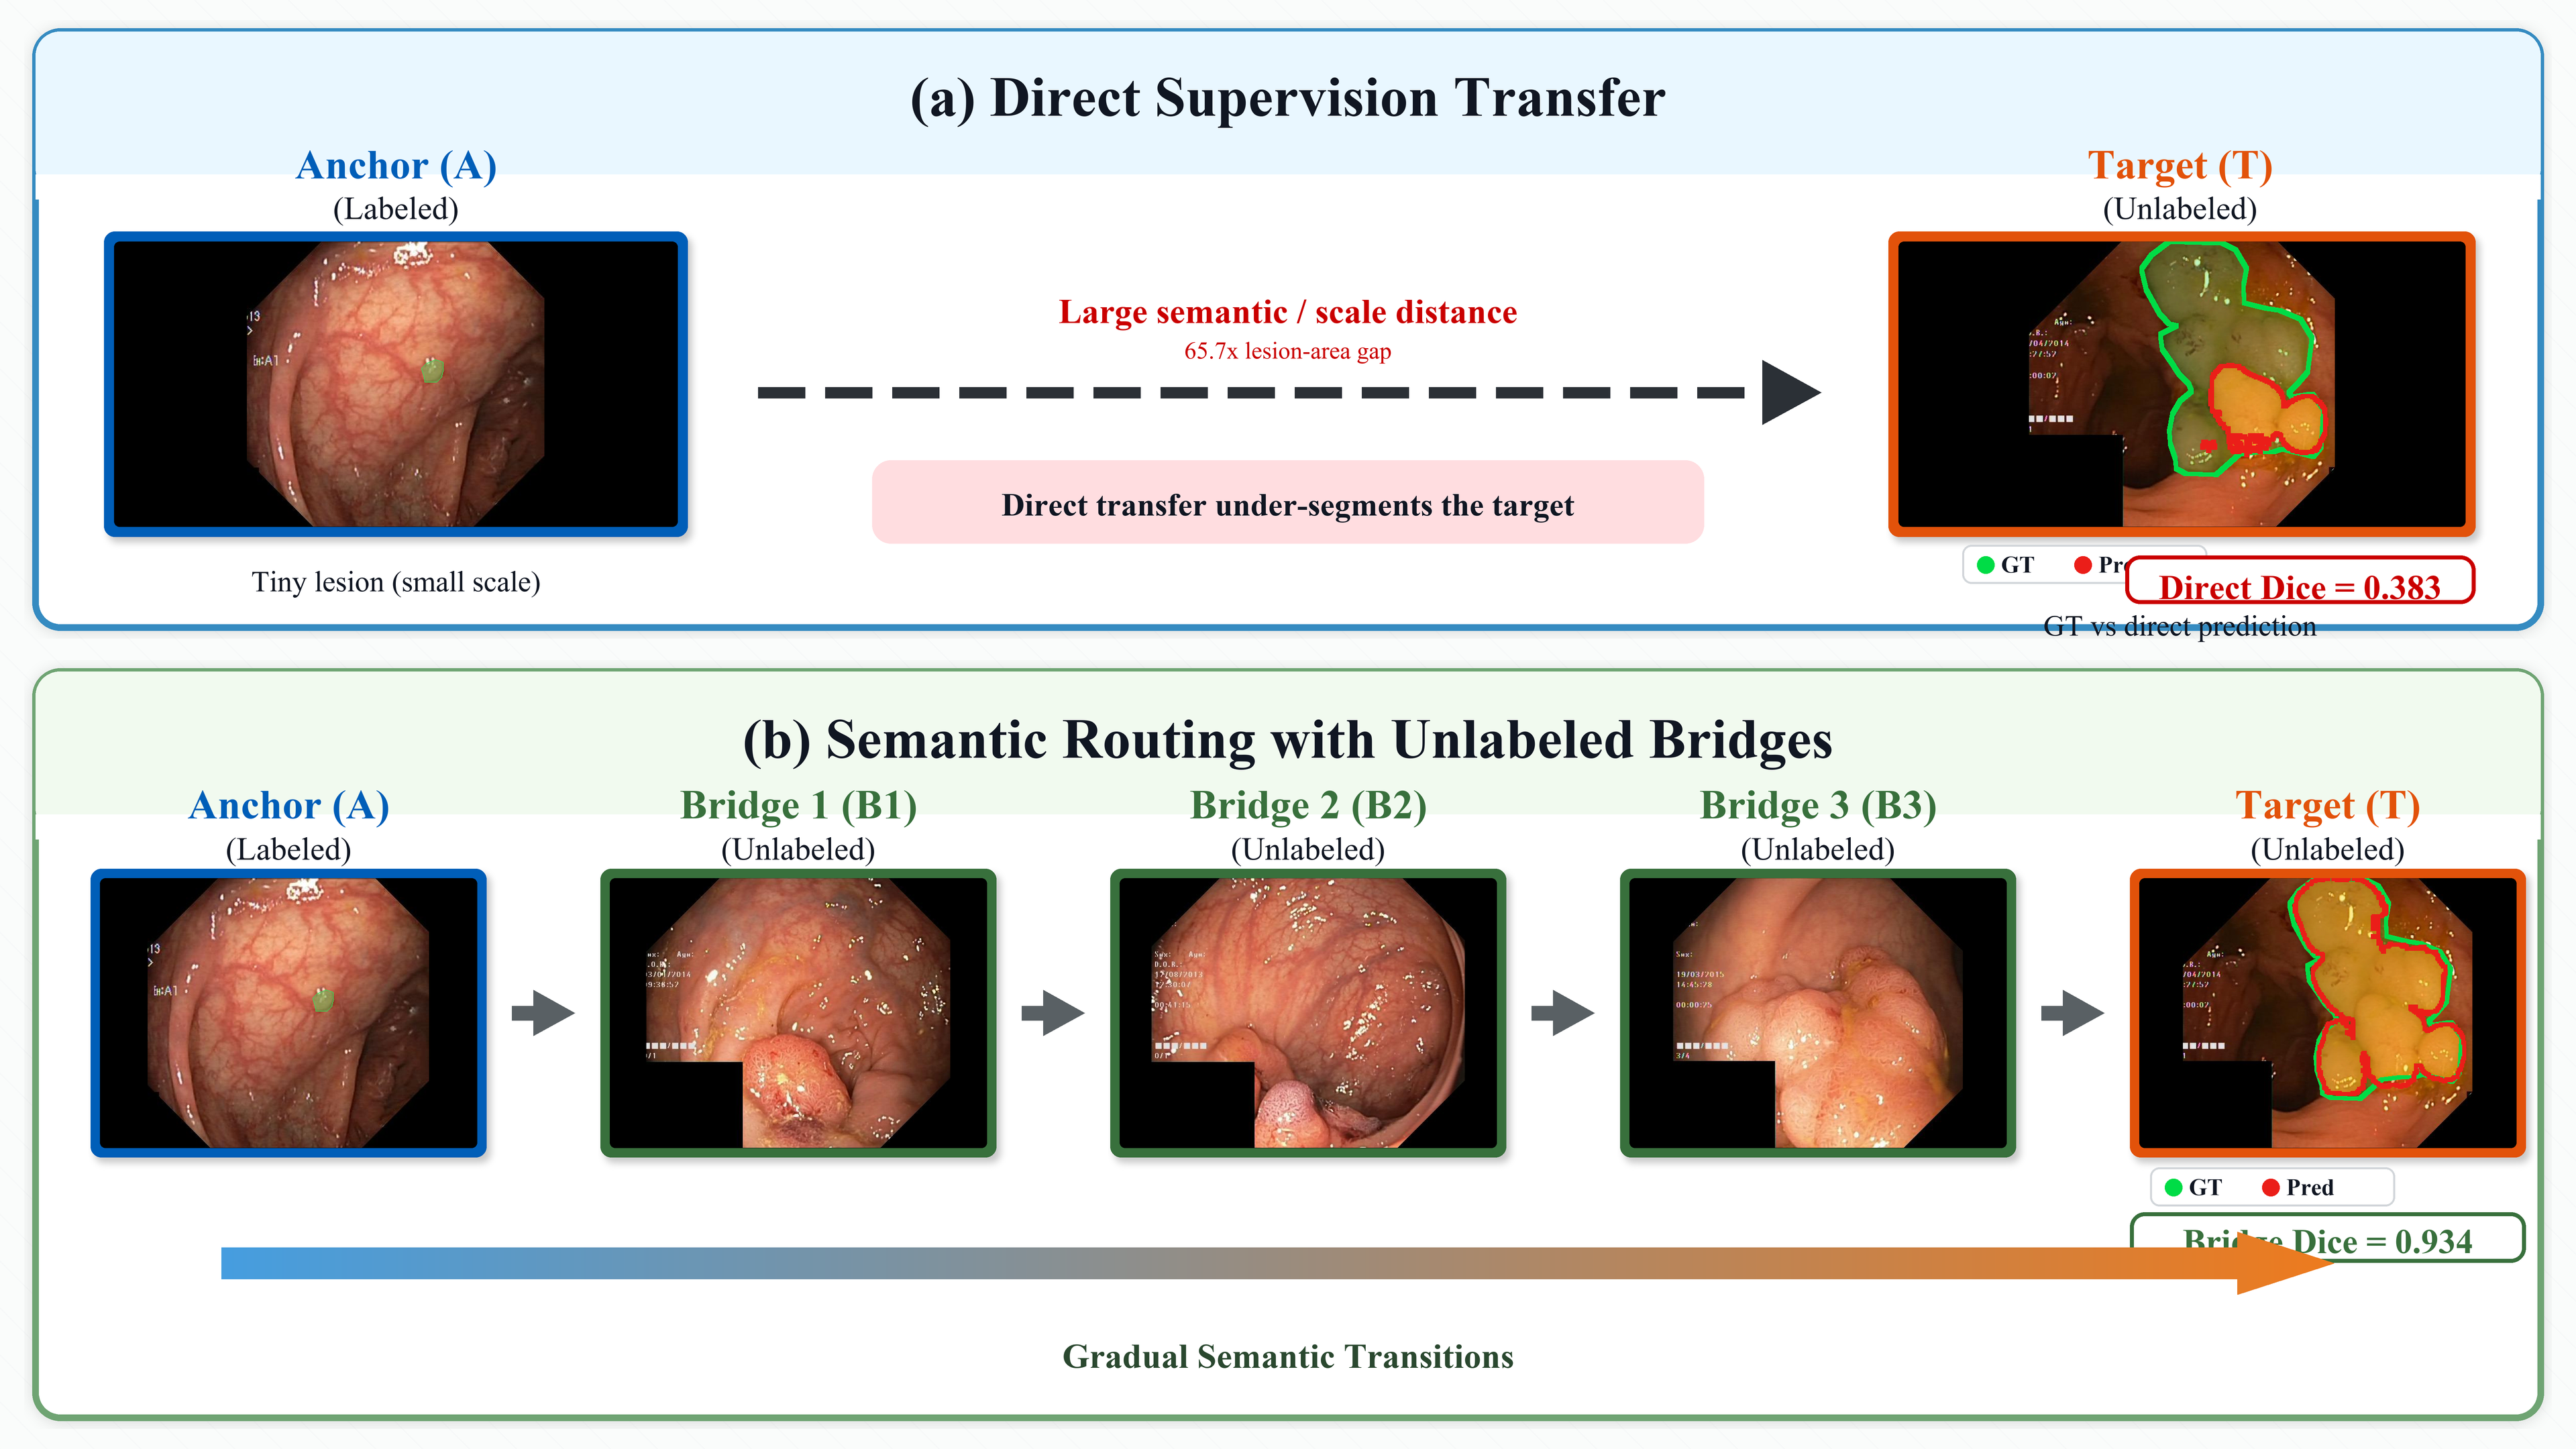
\includegraphics[width=1\linewidth]{figs/figure1.png}
    \caption{Conceptual comparison between direct and routed cross-image propagation. Given a labeled Anchor $A$ and an unlabeled Target $T$, direct propagation transfers the mask in a single source-to-target step. RouteSAM retrieves and orders unlabeled Bridge images $\{B_i\}_{i=1}^{K}$ and applies SAM3 sequentially along $A\rightarrow B_1\rightarrow\cdots\rightarrow B_K\rightarrow T$. The Bridges provide intermediate semantic states that reduce the difficulty of a large one-step transfer. The route is constructed only during training; the final specialist performs direct single-image inference. The displayed masks constitute an illustrative example rather than an aggregate comparison.}
    \label{fig:motivation}
\end{figure}

We instead view the unlabeled medical dataset as both a collection of prediction targets and a semantic transition space. Between a labeled source and a difficult target, the pool may contain images that provide intermediate semantic states and make successive transfers more local. As illustrated in Fig.~\ref{fig:motivation}, this view changes the central question from \emph{how to improve the prediction of each unlabeled image} to \emph{how to design the path through which sparse supervision reaches that image}.

To answer this question, we propose \textbf{RouteSAM}, a semantic-routing framework for semi-supervised 2D medical image segmentation under extreme label scarcity. Given a fixed annotation budget, RouteSAM selects distribution-covering training images as labeled Anchors. For each unlabeled Target, target-conditioned retrieval chooses a suitable Anchor and Bridge candidates, and orders them into an Anchor--Bridge--Target route. SAM3 treats the ordered images as a pseudo-video and progressively propagates the Anchor mask, producing target candidates from different sources and route depths. A route-aware quality model then selects reliable candidates for pseudo supervision. Rather than using the specialist merely as another same-image collaborator, RouteSAM trains a task-specific U-Net to absorb route-derived supervision and audit propagation candidates. Its domain-specific predictions guide parameter-efficient SAM3 adaptation, after which the adapted model re-propagates along the same frozen routes to construct a second-round training set. Route construction is confined to training; the final specialist performs prompt-free, single-image inference.

We evaluate RouteSAM on Kvasir-SEG, BUSI, and ISIC2018 under an approximately 1\% annotation budget. The experiments compare it with conventional SSMIS methods, SAM-assisted approaches, and one-shot propagation baselines, and analyze the effects of Anchor selection, Bridge depth, candidate selection, specialist auditing, SAM3 adaptation, and re-propagation. \textbf{[Final quantitative results will be inserted here after the unified closed-loop evaluation is complete.]}

The main contributions of this work are summarized as follows:
\begin{itemize}
\item We formulate semi-supervised medical image segmentation as a cross-image supervision-routing problem, shifting the focus from independent per-image pseudo-label generation to explicit propagation-path design over the unlabeled training set.

\item We develop a coverage-aware Anchor selection and target-conditioned route-construction strategy that organizes selected unlabeled Bridges into an ordered semantic route, allowing SAM3 to replace a difficult one-step transfer with a sequence of more local propagation steps.

\item We introduce a route-aware supervision pipeline in which SAM3 generates multiple route-dependent candidates, a quality model selects reliable pseudo supervision, and a task-specific specialist audits the candidates and guides route-preserving adaptation and re-propagation while retaining direct single-image inference.
\end{itemize}

\section{Related Work}

\subsection{Semi-Supervised Medical Image Segmentation}

Semi-supervised medical image segmentation learns from limited pixel-level annotations and abundant unlabeled images. A dominant family of methods relies on consistency regularization. Mean Teacher uses an exponential-moving-average teacher to provide stable targets under perturbations~\cite{tarvainen2017meanteacher}. Cross Pseudo Supervision trains two independently initialized networks to exchange hard pseudo labels~\cite{chen2021cps}, while Cross Teaching exploits the complementary inductive biases of CNN and Transformer models~\cite{luo2022crossteaching}. MC-Net+ estimates uncertain regions from multiple decoders and imposes mutual consistency with soft pseudo labels~\cite{wu2022mcnet}.

Recent methods improve the reliability of perturbation-based learning and pseudo supervision. BCP reduces the empirical mismatch between labeled and unlabeled data through bidirectional copy--paste~\cite{bai2023bcp}. ABD uses confidence-guided bidirectional patch displacement to control multiple perturbations~\cite{chi2024abd}, whereas DyCON dynamically reweights uncertain voxels and combines consistency with focal contrastive learning~\cite{assefa2025dycon}. Although these methods exploit unlabeled data effectively, their supervisory mechanisms are mainly defined through predictions, perturbations, or local sample mixing. They do not explicitly construct a multi-image path along which sparse segmentation supervision is propagated.

\subsection{Foundation Model-Assisted Label-Efficient Medical Segmentation}

The promptable Segment Anything Model has motivated the use of foundation-model priors in label-efficient medical segmentation. SemiSAM adds a frozen SAM-assisted branch to a conventional consistency framework, using specialist predictions to generate prompts and SAM outputs as additional supervision~\cite{zhang2023semisam}. SemiSAM+ generalizes this design to one or multiple frozen generalists and introduces confidence-aware specialist--generalist collaboration~\cite{zhang2025semisamplus}. SAMatch combines weak-to-strong Match learning with a task-adapted SAM: the Match teacher generates automatic prompts, and SAM returns refined masks for student training~\cite{xu2024samatch}.

Other methods adapt SAM itself using unlabeled data. CPC-SAM uses two SAM decoders for mutual prompting and supervision, together with a prompt consistency constraint~\cite{miao2024cpcsam}. SC-SAM uses a U-Net to provide point prompts and pseudo labels for efficient SAM adaptation; SAM in turn regularizes the U-Net~\cite{vu2026scsam}. CPPS-SAM transfers knowledge bidirectionally between a CNN expert and a SAM generalist through cross prompting and cross pseudo supervision~\cite{zhang2026cppssam}. These methods establish effective generalist--specialist interaction, but the interaction is primarily performed within individual images. RouteSAM is complementary: it focuses on how supervision is organized and propagated across a sequence of related images.

\subsection{Cross-Image Relation Modeling and Propagation}

Several SSMIS methods exploit relationships among images to improve representation learning. ACTION performs global and local anatomical-aware contrastive distillation~\cite{you2022action}. DACL uses density-aware neighbor graphs to pull sparse features toward high-density class regions~\cite{tang2024dacl}, while GraphCL incorporates instance graphs and graph-based clustering into a teacher--student framework~\cite{wang2024graphcl}. These studies demonstrate that unlabeled medical datasets contain valuable cross-sample structure; however, the learned relations regularize feature geometry rather than define an executable path for segmentation propagation.

Reference-based methods perform more direct cross-image transfer. PerSAM and Matcher personalize or prompt SAM from a reference image and mask~\cite{zhang2023persam,liu2023matcher}, while OP-SAM transfers one-shot polyp priors through support--query correlation and iterative prompt evolution~\cite{mao2025opsam}. YoloSeg uses SAM2 to propagate a single annotation to unlabeled images and trains a specialist using multi-view pseudo-label consensus~\cite{zhang2026yoloseg}. In contrast to these direct or support-conditioned approaches, RouteSAM explicitly selects the propagation source and inserts ordered unlabeled Bridges between the Anchor and Target. The resulting route converts the unlabeled pool from a set of passive prediction targets into an active transition space for progressive supervision transfer.

\section{Method}\label{sec:method}

\subsection{Problem Formulation and Framework Overview}

Let $\mathcal{D}_{\mathrm{tr}}=\{x_i\}_{i=1}^{N}$ denote a training set and let $\mathcal{D}_{\mathrm{val}}$ and $\mathcal{D}_{\mathrm{te}}$ denote fixed validation and test sets. Under an approximately 1\% annotation budget, we select
\begin{equation}
K=\max\left(1,\operatorname{round}(0.01N)\right)
\end{equation}
training images as Anchors and acquire their masks. The remaining training images form an unlabeled pool $\mathcal{U}$. Validation labels are used only to fit and select quality-estimation components, and test labels are withheld until all test predictions are frozen.

RouteSAM contains three stages. Stage~0 selects a coverage-aware Anchor set using training RGB images only. Stage~1 retrieves Anchor and Bridge images for every target, constructs routes of different depths, propagates the Anchor mask with a frozen SAM3, and selects a route-dependent target mask. Stage~2 trains a single-image specialist from the propagated supervision, uses the specialist to audit route candidates and guide SAM3 adaptation, and re-propagates along the frozen routes before training the final deployment model.

\subsection{Coverage-Aware Anchor Selection}\label{sec:anchor-selection}

Because an Anchor is both a labeled example and the starting point of many propagation routes, we select Anchors to cover the training distribution rather than sample them independently. No mask is read before the selected list is frozen.

\paragraph{Global descriptor.}
Each training image is encoded at a resolution of $1008 \times 1008$ by the frozen SAM3 image backbone. Let $\mathbf{P}_i=\{\mathbf{p}_{i,r}\}_{r=1}^{72\times72}$ be its patch tokens. After normalizing every token, the global descriptor is
\begin{equation}
\mathbf{g}_i=\operatorname{norm}\left(\frac{1}{|\mathbf{P}_i|}\sum_r
\operatorname{norm}(\mathbf{p}_{i,r})\right),
\end{equation}
where $\operatorname{norm}(\mathbf{v})=\mathbf{v}/\lVert\mathbf{v}\rVert_2$.

\paragraph{Local descriptor.}
We uniformly sample an $8\times8$ grid of patch tokens from every image and fit a 64-cluster MiniBatch K-Means dictionary on the training split. Let $h_{i,c}$ be the normalized count of visual word $c$ in image $i$, and let
\begin{equation}
\operatorname{idf}_c=\log\frac{N+1}{\operatorname{df}_c+1}+1.
\end{equation}
The local descriptor is the normalized Hellinger-transformed histogram
\begin{equation}
\mathbf{l}_i=\operatorname{norm}\left(\sqrt{\mathbf{h}_i\odot\mathbf{idf}}\right).
\end{equation}
We combine global and local appearance using
\begin{equation}
S(i,j)=\frac{1}{2}\left[\mathbf{g}_i^{\top}\mathbf{g}_j\right]_+
+\frac{1}{2}\left[\mathbf{l}_i^{\top}\mathbf{l}_j\right]_+,
\end{equation}
where $[z]_+=\max(z,0)$.

\paragraph{Greedy coverage.}
For an Anchor set $\mathcal{A}$, the facility-style coverage objective is
\begin{equation}
F(\mathcal{A})=\frac{1}{N}\sum_{i=1}^{N}\max_{a\in\mathcal{A}}S(i,a).
\end{equation}
Starting from the empty set, we repeatedly add the image with the largest marginal gain in $F$ until $K$ Anchors have been selected. Exact image-file duplicates are excluded from the candidate set, while every training image remains part of the coverage objective. Ties are resolved by a fixed sample-ID order. The selected list and its hash are frozen before the corresponding masks are opened.

\subsection{Target-Aware Anchor Retrieval}\label{sec:target-pooling}

Stage~1 uses a separate $256\times256$ representation for retrieval and propagation. The SAM3 backbone produces an $18\times18$ grid of 1024-dimensional patch tokens $\{\mathbf{x}_{i,j}\}_{j=1}^{324}$. For Anchor $a$, its mask is resized to the patch grid and the foreground tokens are averaged to obtain a target prototype
\begin{equation}
\mathbf{p}_a=\operatorname{norm}\left(
\frac{1}{|\Omega_a|}\sum_{j\in\Omega_a}\operatorname{norm}(\mathbf{x}_{a,j})
\right),
\end{equation}
where $\Omega_a$ contains foreground patch positions. If $\Omega_a$ is empty after resizing, the whole-image patch mean is used.

For a target $t$, the similarity between $\mathbf{p}_a$ and each target patch is converted into attention weights
\begin{equation}
w_{a,t,j}=\frac{\exp(\beta\mathbf{p}_a^{\top}\mathbf{x}_{t,j})}
{\sum_k\exp(\beta\mathbf{p}_a^{\top}\mathbf{x}_{t,k})},
\qquad \beta=10.
\end{equation}
The Anchor-conditioned target descriptor and Target Pooling score are
\begin{equation}
\mathbf{z}(a,t)=\operatorname{norm}\left(\sum_jw_{a,t,j}\mathbf{x}_{t,j}\right),
\qquad
r(a,t)=\mathbf{p}_a^{\top}\mathbf{z}(a,t).
\end{equation}
The default retrieval score is $r(a,t)$. We additionally study a centered score $r(a,t)-\mu_a$, where $\mu_a$ is the mean Target Pooling score of Anchor $a$ over training RGB images. Centering changes only Anchor ranking and is treated as a calibration ablation; it does not change the route objective. The highest-ranked one or two Anchors are retained for route construction.

\subsection{Ordered Semantic Route Construction}\label{sec:route-construction}

For every retained Anchor--Target pair, RouteSAM constructs routes with zero to six Bridge images:
\begin{equation}
\mathcal{R}_{b}: A\rightarrow B_1\rightarrow\cdots\rightarrow B_b\rightarrow T,
\qquad b\in\{0,\ldots,6\}.
\end{equation}
All Bridges are drawn only from the training split, and a target is excluded from its own Bridge chain. Consecutive-image affinity is computed by cosine similarity between normalized whole-image patch-mean descriptors. For a candidate route, we collect the Target Pooling scores of its intermediate nodes and target together with its consecutive-edge affinities. The route score is the lexicographic pair
\begin{equation}
Q(\mathcal{R})=\left(\min_{v\in\mathcal{V}(\mathcal{R})}v,
\frac{1}{|\mathcal{V}(\mathcal{R})|}\sum_{v\in\mathcal{V}(\mathcal{R})}v\right),
\end{equation}
which first maximizes the bottleneck value and then the mean value. An independent beam search with width 32 is performed for each depth $b$. This objective favors routes without a severely mismatched node or transition while preserving high average relevance.

\subsection{Progressive SAM3 Propagation}\label{sec:sam3-propagation}

Each route is treated as a short pseudo-video whose frames follow the order in Eq.~(10). SAM3 is initialized on the Anchor using the tight bounding box of its manual mask; no text prompt is used. The model then propagates the object mask through the Bridge frames to the Target on a $256\times256$ canvas. The binary mask on the final Target frame is stored as one route-dependent candidate $\hat{y}_{t,\mathcal{R}}$.

To obtain a label-free propagation-quality signal, we also perform a return pass. The predicted Target mask, never the Target ground truth, initializes backward propagation along the reversed route. Its returned Anchor mask is compared with the known Anchor mask to obtain cycle consistency $q_{\mathrm{cycle}}$. Because the comparison is made only at the labeled Anchor, the feature is available for both unlabeled training targets and held-out targets.

\subsection{Route-Candidate Quality Estimation}\label{sec:router}

Retaining $M$ Anchors yields $7M$ candidates per target. RouteSAM represents each candidate using 28 ground-truth-free features. Seven base features encode route depth, bottleneck and mean route affinity, the final SAM score, candidate count, and depth--affinity interactions. The remaining 21 propagation features describe return consistency and success, mask-area variation, empty masks and connected components, centroid and bounding-box drift, adjacent-frame mask agreement, SAM-score trajectories, and candidate-count trajectories.

We standardize these features and fit a Ridge regressor with $\alpha=1$ to predict candidate Dice on the validation set. Five-fold fitting groups all candidates from the same validation image to prevent candidate-level leakage. At inference, the candidate with the highest predicted quality is selected, with deterministic Anchor-rank and route-depth tie breaking. All test choices are frozen before test ground truth is read. The per-target Oracle over the same candidate pool is reported only as a diagnostic upper bound and is never used for deployment.

\subsection{Specialist Auditing and SAM3 Adaptation}\label{sec:collaboration}

The selected Stage~1 masks form the first-round pseudo-labeled set
\begin{equation}
\widehat{\mathcal{D}}_{U}^{(1)}=\{(x_t,\hat{y}_t^{(1)},q_t^{(1)})\mid x_t\in\mathcal{U}\},
\end{equation}
where $q_t^{(1)}$ is the predicted route quality. A task-specific U-Net $f_{\theta}$ is trained from the Anchor ground truth and accepted pseudo labels. We define
\begin{equation}
\begin{aligned}
\mathcal{L}_{\mathrm{sup}}&=\frac{1}{K}\sum_{a\in\mathcal{A}}
\ell(f_{\theta}(x_a),y_a),\\
\mathcal{L}_{\mathrm{pseudo}}&=\frac{1}{|\widehat{\mathcal{D}}_{U}^{(1)}|}
\sum_t q_t^{(1)}\ell(f_{\theta}(x_t),\hat{y}_t^{(1)}),\\
\mathcal{L}_{\mathrm{student}}&=\mathcal{L}_{\mathrm{sup}}
+\lambda_u\mathcal{L}_{\mathrm{pseudo}},
\end{aligned}
\end{equation}
where $\ell$ combines binary cross-entropy and soft Dice losses.

The specialist then acts as an independent auditor of SAM3 propagation. For every route candidate, we combine the propagation-quality estimate with its agreement to the specialist prediction. Candidate acceptance thresholds and combination weights are chosen only on the validation set. Unlike same-image specialist--generalist co-training, this audit operates on a set of masks produced by different cross-image routes and can therefore identify routes that are self-consistent but inconsistent with target-domain appearance.

Accepted Anchor masks and audited pseudo labels are used for parameter-efficient SAM3 adaptation. To isolate model adaptation from route search, the Anchor identity, Bridge membership, route order, and candidate policy are frozen before this update.

% TODO(Stage 2): freeze the exact audit formula, thresholds, PEFT modules, and
% optimization schedule after the automatic-Anchor closed loop is implemented.

\subsection{Route-Preserving Re-Propagation and Final Inference}\label{sec:repropagation}

The adapted SAM3 is applied to the same frozen routes to obtain second-round candidates $\hat{y}_{t,\mathcal{R}}^{(2)}$. The quality estimator and specialist audit are then applied under the pre-specified validation policy to construct $\widehat{\mathcal{D}}_{U}^{(2)}$. A final U-Net is trained from the Anchor ground truth and this second-round pseudo supervision using the objective in Eq.~(13).

Semantic retrieval and SAM3 propagation are training-time mechanisms. At test time, the final U-Net receives only a single image and directly predicts its segmentation mask. It does not retrieve an Anchor, construct a route, or require a manual prompt. This separation allows RouteSAM to use expensive cross-image reasoning for supervision expansion while retaining a lightweight deployment path.

% To print the credit authorship contribution details
\printcredits

%% Loading bibliography style file
%\bibliographystyle{model1-num-names}
\bibliographystyle{cas-model2-names}

% Loading bibliography database
\bibliography{related_work_papers/references}

% Biography
%\bio{}
% Here goes the biography details.
%\endbio

%\bio{pic1}
% Here goes the biography details.
%\endbio

\end{document}
